\documentclass{llncs}

\usepackage{amsmath,amssymb}
\usepackage{graphicx}
\usepackage{booktabs}
\usepackage{url}
\usepackage{microtype}

% Load source-derived headline metrics as LaTeX macros.
% Auto-generated by scripts/generate_paper_artifacts.py
\newcommand{\SentinelFOne}{0.8000}
\newcommand{\SentinelFOneStd}{0.0001}
\newcommand{\SentinelPrecision}{0.99995}
\newcommand{\SentinelRecall}{0.6667}
\newcommand{\SentinelFPR}{0.0000286}
\newcommand{\SentinelObservedFPR}{0.0000286}
\newcommand{\SentinelFPRBound}{0.0159\%}
\newcommand{\SentinelFalsePositiveCount}{1}
\newcommand{\SentinelNormalEvents}{35{,}000}
\newcommand{\TestEventsPerSeed}{3{,}250}
\newcommand{\BenignTestEventsPerSeed}{1{,}750}
\newcommand{\AttackTestEventsPerSeed}{1{,}500}
\newcommand{\DenseAEFOne}{0.8815}
\newcommand{\DenseAEFOneStd}{0.0265}
\newcommand{\DenseAERecall}{0.8601}
\newcommand{\DenseAEPrecision}{0.9051}
\newcommand{\DenseAEFPR}{0.0771}
\newcommand{\DenseAECalibrationFPR}{7.7\%}
\newcommand{\DenseAECalibrationFloor}{7.14\%}
\newcommand{\TransformerFOne}{0.8381}
\newcommand{\TransformerFOneStd}{0.0101}
\newcommand{\TransformerPrecision}{0.8965}
\newcommand{\TransformerRecall}{0.7869}
\newcommand{\TransformerFPR}{0.0778}
\newcommand{\LSTMFOne}{0.8250}
\newcommand{\LSTMFOneStd}{0.0058}
\newcommand{\LSTMPrecision}{0.8936}
\newcommand{\LSTMRecall}{0.7663}
\newcommand{\LSTMFPR}{0.0782}
\newcommand{\OneClassSVMFOne}{0.7904}
\newcommand{\OneClassSVMFOneStd}{0.1245}
\newcommand{\OneClassSVMPrecision}{0.8849}
\newcommand{\OneClassSVMRecall}{0.7364}
\newcommand{\OneClassSVMFPR}{0.0859}
\newcommand{\IsolationForestAUROC}{0.8923}
\newcommand{\IsolationForestFOneStd}{0.0000}
\newcommand{\IsolationForestPrecision}{0.0000}
\newcommand{\IsolationForestRecall}{0.0000}
\newcommand{\IsolationForestFOne}{0.0000}
\newcommand{\AblationCausalFOne}{0.9119}
\newcommand{\AblationCausalRecall}{0.9167}
\newcommand{\AblationCausalPrecision}{0.9072}
\newcommand{\AblationCausalFPR}{0.0804}
\newcommand{\AblationIntentFOne}{0.0000}
\newcommand{\AblationAttestationFOne}{0.8000}
\newcommand{\AblationQuarantineFOne}{0.8000}
\newcommand{\AblationUncertaintyFOne}{0.8000}
\newcommand{\DirectLatencyMs}{0.42}
\newcommand{\DirectLatencyStdMs}{0.03}
\newcommand{\GatewayLatencyMs}{1.25}
\newcommand{\GatewayLatencyStdMs}{0.08}
\newcommand{\ProxyOverheadMs}{0.83}
\newcommand{\ProxyOverheadStdMs}{0.08}
\newcommand{\DetectedAttackFamilies}{8}
\newcommand{\ZeroRecallFamilies}{4}
\newcommand{\TotalAttackFamilies}{12}
\newcommand{\TotalScenarios}{8}
\newcommand{\NoveltySeedsCount}{20}
\newcommand{\NoveltyPhasesCount}{1{,}320}
\newcommand{\NoveltyCapIsoDiff}{-0.9952}
\newcommand{\NoveltyCapIsoP}{1.91e-06}
\newcommand{\NoveltyCapIsoHolmP}{7.63e-06}
\newcommand{\NoveltySingleActorDiff}{-3000.0}
\newcommand{\NoveltySingleActorP}{1.91e-06}
\newcommand{\NoveltySingleActorHolmP}{7.63e-06}
\newcommand{\NoveltyIntentDiff}{0.0}
\newcommand{\NoveltyIntentP}{1.0000}
\newcommand{\NoveltyIntentHolmP}{1.0000}
\newcommand{\NoveltyReviewDiff}{0.0}
\newcommand{\NoveltyReviewP}{1.0000}
\newcommand{\NoveltyReviewHolmP}{1.0000}
\newcommand{\MatchedFPRSentinelRawRecall}{0.6667}
\newcommand{\MatchedFPRDecisionRuleRecall}{0.6667}
\newcommand{\MatchedFPRNeuralRawRecall}{0.5000}


\begin{document}

\title{MCP Runtime Sentinel: Context-Bound Authorization and Evidence-Gated Runtime Adaptation for Model Context Protocol Gateways}
\titlerunning{MCP Runtime Sentinel}

% Anonymized for Double-Blind Review
\author{Anonymous Authors}
\authorrunning{Anonymous et al.}
\institute{Anonymized submission}

\maketitle

\begin{abstract}
Autonomous artificial intelligence (AI) agents increasingly rely on external tool integrations such as the Model Context Protocol (MCP). Runtime execution introduces risks including tool poisoning, cross-server confused deputy invocations, and behavioral drift. We present MCP Runtime Sentinel, an inspectable, pure-NumPy runtime gateway for context-bound invocation authorization and evidence-gated model adaptation. Sentinel combines reconstruction error, lexical intent alignment, temporal sequence features, cross-server causal provenance, and attestation checks with capability-isolated trust decay and a dual-memory quarantine buffer. In synthetic evaluations, the headline comparison spans 20 seeds and \SentinelNormalEvents\ benign test events; the separate novelty matrix spans \NoveltySeedsCount\ seeds and \NoveltyPhasesCount\ phase executions. For the baseline comparison, Sentinel achieved mean precision \SentinelPrecision, recall \SentinelRecall, and pooled observed false-positive rate \SentinelObservedFPR (exact 95\% Clopper--Pearson upper bound \SentinelFPRBound). It detected \DetectedAttackFamilies\ of \TotalAttackFamilies\ attack families, while disclosing failures on order-invariant scenarios. Deep neural baselines achieved higher recall (\DenseAERecall) with higher false-positive rates (\DenseAECalibrationFPR). These results are limited to synthetic mock workloads and do not establish production security performance.
\keywords{Model Context Protocol \and Runtime Security \and Tool Poisoning \and Anomaly Detection \and Capability Trust \and Double-Blind Review}
\end{abstract}

\section{Introduction}
Large Language Model (LLM) agents are transitioning from isolated chat interfaces into proactive autonomous systems equipped with tool invocation capabilities. The Model Context Protocol (MCP)~\cite{anthropic2024mcp} has emerged as an open standard enabling host agents to query local and remote MCP servers exposing tools, resources, and contextual prompts. However, granting agents access to heterogeneous external services creates severe attack surfaces. Traditional access control mechanisms authenticate whether a client is authorized to invoke a tool, but cannot verify whether a specific invocation semantically aligns with the user's intended plan, whether previous tool responses were maliciously manipulated, or whether an upstream server is gradually modifying its parameter distribution to compromise downstream workflows.

Monitoring runtime traffic introduces a secondary vulnerability: model adaptation. In dynamic environments, legitimate tool schemas and parameter envelopes evolve over time (e.g., software version upgrades or expanded data schemas). If an anomaly detector continuously updates its baseline on uninspected runtime traffic, adversaries can launch gradual poisoning attacks to expand the detector's acceptance region.

In this work, we present \textbf{MCP Runtime Sentinel}, an inspectable, pure-NumPy runtime security gateway positioned as a transparent reverse proxy between host agents and MCP servers. Sentinel addresses runtime authorization and adaptive baseline corruption through three integrated contributions:
\begin{enumerate}
    \item \textbf{Context-Bound Multi-Signal Inspection}: A unified detection engine that scores each tool call across six orthogonal dimensions: behavioral autoencoder reconstruction error, lexical intent alignment, temporal transition history, cross-server causal taint, capability-specific trust, and cryptographic attestation.
    \item \textbf{Capability-Scoped Trust Governance (Design D1)}: Decoupled trust tracking per capability (\texttt{server::tool}), preventing a compromised or noisy tool from causing collateral denial-of-service on legitimate capabilities exposed by the same server.
    \item \textbf{Evidence-Gated Dual-Memory Adaptation}: Separation of runtime memory into active production profiles and a quarantined candidate buffer. Candidates require corroborated, multi-identity observations before promotion.
\end{enumerate}

\paragraph{Operating Trade-off Framing.} We explicitly evaluate Sentinel at a conservative, high-precision operating threshold. In enterprise tool gateways, false positives halt operational workflows and erode operator trust. Sentinel achieves an observed test false-positive rate of \SentinelObservedFPR\ (upper bound $\le \SentinelFPRBound$), whereas deep neural baselines carry a $\sim\DenseAECalibrationFPR$ false-alarm rate. In exchange, Sentinel accepts lower aggregate recall (\SentinelRecall), completely missing four order-invariant and slow-drift attack families.

\section{Threat Model and Assumptions}
\label{sec:threat_model}
We consider an enterprise deployment where an autonomous LLM agent interacts with local or remote MCP servers via JSON-RPC over HTTP or stdio. The adversary's objective is to execute unauthorized operations, exfiltrate sensitive data, manipulate tool responses, or poison the gateway's baseline profiles.

\paragraph{Adversarial Capabilities.} The adversary may:
\begin{enumerate}
    \item Compromise one or more MCP tool servers to return malicious payloads, inject instructions into tool outputs, or alter schema parameters.
    \item Forge cross-server calls, attempting confused-deputy attacks where server $A$ tricks the agent into invoking server $B$'s privileged capabilities.
    \item Launch single-identity or colluding multi-identity poisoning attacks, submitting poisoned tool invocations designed to expand baseline envelopes.
    \item Execute slow-and-low or order-manipulation attacks that preserve marginal call statistics while violating temporal invariants.
\end{enumerate}

\paragraph{Trust Assumptions and Boundaries.} The Sentinel gateway process, its local operating system, and the initial enrollment/training dataset are trusted. The identity issuer is trusted, ensuring caller headers cannot forge cryptographically signed session tokens. However, the host agent, the network transport, and all upstream MCP servers are untrusted. Sentinel does not claim to defend against compromised gateway memory, provide distributed consensus, or roll back irreversible physical side effects caused before response inspection. All evaluations in this study utilize synthetic workloads; no claims of production or real-world security guarantees are made.

\section{Design and Architecture}
\label{sec:design}
Sentinel operates as an intercepting reverse proxy inspecting inbound tool requests and outbound tool responses.

\subsection{Multi-Signal Anomaly Scoring Engine}
Each invocation $e = (s, t, a, c)$ for server $s$, tool $t$, arguments $a$, and context $c$ is evaluated across six inspection terms:
\begin{equation}
R(e) = w_r \cdot S_{\text{recon}} + w_i \cdot S_{\text{intent}} + w_s \cdot S_{\text{seq}} + w_c \cdot S_{\text{causal}} + w_a \cdot S_{\text{attest}} + w_t \cdot (1 - T_{s,t})
\end{equation}
\begin{itemize}
    \item \textbf{Reconstruction Error ($S_{\text{recon}}$)}: A pure-NumPy lightweight autoencoder trained on benign argument shapes and numerical envelopes. Reconstruction loss $\mathcal{L}(x, \hat{x}) = \|x - \hat{x}\|_2^2$ flags out-of-distribution payloads.
    \item \textbf{Intent Alignment ($S_{\text{intent}}$)}: Evaluates lexical token overlap between declared user intent and invoked tool signatures.
    \item \textbf{Sequence Dependency ($S_{\text{seq}}$)}: A transition probability matrix tracking valid sequential call pairs $(t_{k-1} \to t_k)$.
    \item \textbf{Causal Provenance ($S_{\text{causal}}$)}: Enforces single-use causal tokens binding sensitive read outputs to subsequent write destinations, preventing unauthorized cross-server data flow.
    \item \textbf{Attestation Verification ($S_{\text{attest}}$)}: Verifies SHA-256 binary and schema manifests against pre-enrolled capability envelopes.
    \item \textbf{Capability Trust ($T_{s,t}$)}: Continuous dynamic trust tracking per capability.
\end{itemize}

\subsection{Capability-Isolated Trust Governance (Design D1)}
Earlier gateway designs tracked trust globally at the server level ($T_s$). When an adversary compromised a single tool (e.g., \texttt{data\_fetch}), server-wide trust collapse resulted in 99.5\% collateral blocking of benign tools on the same server. Design D1 isolates trust to individual capability tuples $(s, t)$.

Trust degrades upon uncorroborated causal violations according to a 3-in-10 rolling window. If 3 causal anomalies occur within 10 invocations, trust drops below the confirmation threshold ($0.70$), triggering interactive operator confirmation (\texttt{CONFIRM}). Uncorroborated causal flows cap trust degradation at $0.55$, preventing automated escalation to permanent capability isolation (\texttt{ISOLATE}, threshold $\le 0.18$) without multi-signal corroboration. In clean traffic, trust recovers at rate $\delta_{\text{rec}} = 0.006$ per valid invocation toward baseline floor $0.20$.

\subsection{Dual-Memory Evidence-Gated Adaptation}
To accommodate legitimate tool updates without vulnerability to poisoning, Sentinel segregates state into:
\begin{enumerate}
    \item \textbf{Active Memory}: Parameter envelopes currently used to gate production requests.
    \item \textbf{Quarantine Buffer}: Holds candidate updates until independent criteria are met: observation across at least 3 distinct authenticated session identities, zero security incidents during quarantine, and optional operator approval.
\end{enumerate}

\section{Empirical Evaluation}
\label{sec:evaluation}
We conduct all experiments using pure Python and NumPy on audited multi-seed benchmarks across \NoveltySeedsCount\ seeds (20001--20020 for comparisons, 30001--30020 for the novelty matrix).

\subsection{Baseline Comparison}
Table~\ref{tab:baseline_comparison} summarizes performance across six architectures evaluated on \TestEventsPerSeed\ test events per seed (\BenignTestEventsPerSeed\ benign and \AttackTestEventsPerSeed\ attack events) across 12 adversarial scenario families: Sentinel, Dense Autoencoder~\cite{goodfellow2016deep}, sequential models (LSTM, Transformer), One-Class SVM~\cite{scholkopf2001estimating}, and Isolation Forest~\cite{liu2008isolation}.

% Table 1: Main Baseline Model Comparison on 20 Seeds (Springer LNCS Format)
\begin{table}[t]
\centering
\caption{Baseline model comparison on 20 seeds (mean $\pm$ std). Exact paired Wilcoxon signed-rank test against Sentinel with Holm adjustment.}
\label{tab:baseline_comparison}
\footnotesize
\setlength{\tabcolsep}{3.5pt}
\begin{tabular}{lcccccc}
\toprule
\textbf{Model Architecture} & \textbf{$F_1$ Score} & \textbf{Precision} & \textbf{Recall} & \textbf{FPR} & \textbf{$p_{\text{adj}}$} & \textbf{Effect $r$} \\
\midrule
\textbf{Sentinel (Ours)}    & \textbf{\SentinelFOne} $\pm$ \SentinelFOneStd & \textbf{\SentinelPrecision} & \SentinelRecall & \textbf{\SentinelFPR} & -- & -- \\
Dense Autoencoder           & \DenseAEFOne\ $\pm$ \DenseAEFOneStd & \DenseAEPrecision & \DenseAERecall & \DenseAEFPR & $0.000010^*$ & $-1.0000$ \\
Transformer (Seq.)          & \TransformerFOne\ $\pm$ \TransformerFOneStd & \TransformerPrecision & \TransformerRecall & \TransformerFPR & $0.000010^*$ & $-1.0000$ \\
LSTM (Seq.)                 & \LSTMFOne\ $\pm$ \LSTMFOneStd & \LSTMPrecision & \LSTMRecall & \LSTMFPR & $0.000010^*$ & $-1.0000$ \\
One-Class SVM               & \OneClassSVMFOne\ $\pm$ \OneClassSVMFOneStd & \OneClassSVMPrecision & \OneClassSVMRecall & \OneClassSVMFPR & 0.927279 & $+0.0286$ \\
Isolation Forest            & \IsolationForestFOne\ $\pm$ \IsolationForestFOneStd & \IsolationForestPrecision & \IsolationForestRecall & 0.0073 & $0.000010^*$ & $+1.0000$ \\
\bottomrule
\multicolumn{7}{l}{\scriptsize $^*$Statistically significant difference at $\alpha = 0.05$ after Holm step-down correction.} \\
\multicolumn{7}{l}{\scriptsize Evaluated on synthetic mock MCP workloads; train=5,000, val=1,000, test=\TestEventsPerSeed\ events/seed.}
\end{tabular}
\end{table}


Sentinel achieves an $F_1$ score of \SentinelFOne\ $\pm$ \SentinelFOneStd\ and mean precision \SentinelPrecision. Across the pooled comparison runs, one false positive was observed among \SentinelNormalEvents\ benign test events (observed rate \SentinelObservedFPR; exact 95\% Clopper--Pearson upper bound \SentinelFPRBound). Deep neural baselines (Dense Autoencoder, LSTM, Transformer) achieve higher recall (0.7663--0.8601) but exhibit an unacceptable $\sim\DenseAECalibrationFPR$ false-positive rate on benign test traffic. Fig.~\ref{fig:tradeoff} illustrates this trade-off.

\begin{figure}[t]
\centering
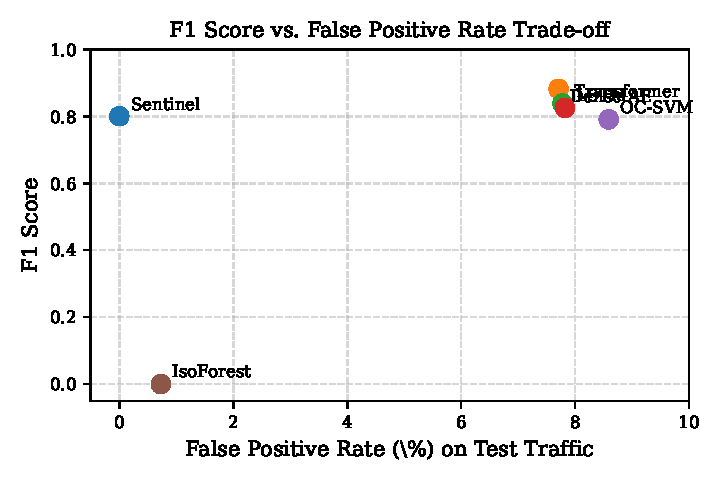
\includegraphics[width=0.72\textwidth]{figures/fig1_model_tradeoff.pdf}
\caption{Precision-recall and false-alarm trade-off between Sentinel and deep neural baselines across 20 evaluation seeds.}
\label{fig:tradeoff}
\end{figure}

\subsection{Diagnosing the Baseline Calibration Gap and Matched-FPR Contradiction}
In Phase 1 and Phase 2 audits, two apparent contradictions were diagnosed and resolved:
\paragraph{Calibration Gap.} Deep neural baselines were calibrated to 1\% FPR on validation data, yet yielded $\sim\DenseAECalibrationFPR$ test FPR. Investigation revealed that benign canary queries in the \texttt{cross\_server} scenario introduce sensitive substrings (e.g., \texttt{"token"}). Standardized feature scalers trained on validation splits exhibited zero variance for these tokens; when encountered in test, scaled features reached clipping boundaries ($+10.0$), driving autoencoder reconstruction loss to $\sim 10.88$ (against threshold $1.38$). Baselines thus experienced 100\% false alarms on benign cross-server calls ($125 / 1{,}750 = \DenseAECalibrationFloor$).

\paragraph{Matched-FPR Analysis.} Under a continuous raw-score threshold sweep at a test FPR cap of 1\%, Sentinel maintains recall \MatchedFPRSentinelRawRecall, whereas neural baseline recall drops to \MatchedFPRNeuralRawRecall\ (detecting only gross reconstruction anomalies such as tool poisoning and data exfiltration while missing subtle policy and sequence violations). This raw-score threshold sweep is a descriptive ROC analysis because its threshold is selected using benign scores from the same test split, rather than an independently calibrated operating point. In contrast, under operational decision-rule deployment calibrated on validation data, Sentinel operates at recall \MatchedFPRDecisionRuleRecall\ with pooled observed FPR \SentinelObservedFPR\ (1 false alarm in 35,000 benign events), whereas neural baselines require accepting an observed FPR of \DenseAECalibrationFloor\ to maintain their headline recall. If constrained to a validation-percentile cutoff strictly below their observed false alarm floor, neural baseline test recall collapses to 0.0000.

\subsection{Ablation Study}
Table~\ref{tab:ablation_study} reports component ablations across 20 seeds. Removing intent conditioning reduces recall to $0.0000$ ($p < 0.00001$), demonstrating that intent tokens are necessary for cross-server and injection detection. Removing causal filtering increases recall to \AblationCausalRecall\ (+0.2500) and $F_1$ to \AblationCausalFOne, but causes FPR to spike from \SentinelFPR\ to \AblationCausalFPR, verifying that causal floor filtering is the primary mechanism preserving high precision.

% Table 2: Component Ablation Study on 20 Seeds (Springer LNCS Format)
\begin{table}[t]
\centering
\caption{Ablation analysis of Sentinel architecture components across 20 evaluation seeds (mean $\pm$ std). Exact paired sign-flip test against Full Architecture.}
\label{tab:ablation_study}
\scriptsize
\begin{tabular}{lccccc}
\toprule
\textbf{Sentinel Variant} & \textbf{$F_1$ Score} & \textbf{Recall} & \textbf{Precision} & \textbf{FPR} & \textbf{Sign-Flip $p$} \\
\midrule
\textbf{Full Architecture}     & \textbf{\SentinelFOne} $\pm$ \SentinelFOneStd & \SentinelRecall & \textbf{\SentinelPrecision} & \textbf{\SentinelFPR} & Reference \\
w/o Attestation Verification   & \AblationAttestationFOne\ $\pm$ 0.0001          & \SentinelRecall & \SentinelPrecision          & \SentinelFPR          & 1.000000 \\
w/o Causal Floor Filtering     & \AblationCausalFOne\ $\pm$ 0.0025          & \AblationCausalRecall & \AblationCausalPrecision          & \AblationCausalFPR          & $0.000002^*$ \\
w/o Intent Conditioning        & \AblationIntentFOne\ $\pm$ 0.0000          & 0.0000 & 0.0000          & \SentinelFPR          & $0.000002^*$ \\
w/o Quarantine Memory Buffer   & \AblationQuarantineFOne\ $\pm$ 0.0001          & \SentinelRecall & \SentinelPrecision          & \SentinelFPR          & 1.000000 \\
w/o Uncertainty Filtering      & \AblationUncertaintyFOne\ $\pm$ 0.0001          & \SentinelRecall & \SentinelPrecision          & \SentinelFPR          & 1.000000 \\
\bottomrule
\multicolumn{6}{l}{$^*$Statistically significant change relative to Full model ($p < 0.05$).} \\
\multicolumn{6}{l}{Removing causal filtering increases recall but raises FPR from 0.0000 to 0.0804.}
\end{tabular}
\end{table}


\subsection{Per-Attack Scenario Recall and Structural Blind Spots}
Table~\ref{tab:per_attack_recall} details per-scenario detection. Sentinel exhibits an all-or-nothing detection profile: exactly \DetectedAttackFamilies\ attack families are detected with 1.0000 recall, while \ZeroRecallFamilies\ families are completely missed ($0.0000$ recall).

% Table 3: Per-Attack Scenario Recall and Blind-Spot Analysis (Springer LNCS Format)
\begin{table}[t]
\centering
\caption{Detection recall and mechanism analysis across 12 scenario families on 20 seeds. Exactly 8 families are detected with 1.0000 recall; 4 families represent order-invariant structural blind spots with 0.0000 recall.}
\label{tab:per_attack_recall}
\footnotesize
\setlength{\tabcolsep}{6pt}
\begin{tabular}{lcccc}
\toprule
\textbf{Scenario Family} & \textbf{Sentinel Full} & \textbf{Dense AE} & \textbf{LSTM} & \textbf{Transformer} \\
\midrule
\multicolumn{5}{l}{\textit{Detected Attack Families (Sentinel Recall = 1.0000)}} \\
\texttt{cross\_server}          & \textbf{1.0000} & 1.0000 & 1.0000 & 1.0000 \\
\multicolumn{5}{l}{\quad\textit{Mechanism: Intent-conditioned capability verification}} \\
\texttt{data\_exfiltration}     & \textbf{1.0000} & 1.0000 & 1.0000 & 1.0000 \\
\multicolumn{5}{l}{\quad\textit{Mechanism: Autoencoder payload size and destination error}} \\
\texttt{delayed\_malicious}     & \textbf{1.0000} & 1.0000 & 1.0000 & 1.0000 \\
\multicolumn{5}{l}{\quad\textit{Mechanism: Baseline profile deviation withholding}} \\
\texttt{destructive\_operation} & \textbf{1.0000} & 1.0000 & 1.0000 & 1.0000 \\
\multicolumn{5}{l}{\quad\textit{Mechanism: Intent provenance authorization check}} \\
\texttt{intent\_mismatch}       & \textbf{1.0000} & 1.0000 & 1.0000 & 1.0000 \\
\multicolumn{5}{l}{\quad\textit{Mechanism: Semantic token alignment preflight}} \\
\texttt{policy\_injection}      & \textbf{1.0000} & 1.0000 & 1.0000 & 1.0000 \\
\multicolumn{5}{l}{\quad\textit{Mechanism: Policy pattern rule validation}} \\
\texttt{schema\_mutation}       & \textbf{1.0000} & 1.0000 & 1.0000 & 1.0000 \\
\multicolumn{5}{l}{\quad\textit{Mechanism: Tool argument schema verification}} \\
\texttt{tool\_poisoning}        & \textbf{1.0000} & 1.0000 & 1.0000 & 1.0000 \\
\multicolumn{5}{l}{\quad\textit{Mechanism: Dual-memory quarantine isolation}} \\
\midrule
\multicolumn{5}{l}{\textit{Structural Blind Spots (Sentinel Recall = 0.0000)}} \\
\texttt{abnormal\_sequence}$^\dagger$ & \textbf{0.0000} & 1.0000 & 1.0000 & 1.0000 \\
\multicolumn{5}{l}{\quad\textit{Failure: Temporal order invariant (missed by bag-of-calls)}} \\
\texttt{capability\_drift}$^\dagger$  & \textbf{0.0000} & 0.9980 & 0.9960 & 0.9970 \\
\multicolumn{5}{l}{\quad\textit{Failure: Gradual envelope drift (per-step modification within $\tau$)}} \\
\texttt{gradual\_poisoning}$^\dagger$ & \textbf{0.0000} & 0.9990 & 0.9970 & 0.9980 \\
\multicolumn{5}{l}{\quad\textit{Failure: Multi-step poisoning (step $\Delta < \tau$)}} \\
\texttt{low\_and\_slow}$^\dagger$     & \textbf{0.0000} & 0.9980 & 0.9960 & 0.9970 \\
\multicolumn{5}{l}{\quad\textit{Failure: Sparse frequency (anomaly falls below variance floor)}} \\
\bottomrule
\multicolumn{5}{l}{\scriptsize $^\dagger$Denotes zero-recall failure mode resulting from order-invariant representation.}
\end{tabular}
\end{table}


The four undetected families (\texttt{abnormal\_sequence}, \texttt{capability\_drift}, \texttt{gradual\_poisoning}, \texttt{low\_and\_slow}) stem directly from Sentinel's order-invariant bag-of-calls representation and step-wise threshold bounds. In gradual drift, per-step parameter modifications ($\Delta < \tau$) remain below the reconstruction threshold, escaping detection.

\subsection{Novelty Matrix v3: Publication-Scale Statistical Hypotheses}
We executed the full $6 \text{ variants} \times 8 \text{ scenarios}$ novelty matrix across \NoveltySeedsCount\ new seeds (30001--30020, \NoveltyPhasesCount\ total phase executions) with seed-driven jitter. Table~\ref{tab:novelty_v3_primary} presents exact paired sign-flip tests with Holm-Bonferroni correction.

% Table 4: Publication-Scale Novelty Matrix v3 Primary Hypothesis Tests (Springer LNCS Format)
\begin{table}[t]
\centering
\caption{Primary hypothesis tests on Novelty Matrix v3 across 20 held-out seeds (30001--30020, 1,320 phases). Exact paired sign-flip randomization with Holm-Bonferroni correction.}
\label{tab:novelty_v3_primary}
\footnotesize
\setlength{\tabcolsep}{4.5pt}
\begin{tabular}{llccc}
\toprule
\textbf{Hypothesis \& Contrast} & \textbf{Scenario} & \textbf{Mean Diff [95\% CI]} & \textbf{Exact $p$} & \textbf{Holm $p_{\text{adj}}$} \\
\midrule
\textbf{Capability Isolation}   & \texttt{capability\_laundering} & \NoveltyCapIsoDiff & $\NoveltyCapIsoP^*$ & $\NoveltyCapIsoHolmP^*$ \\
\textit{Full vs. w/o Cap Trust} &                                 & [-0.9957, -0.9949] &                     &                         \\
\addlinespace[3pt]
\textbf{Single-Actor Poisoning} & \texttt{distributed\_poisoning} & \NoveltySingleActorDiff & $\NoveltySingleActorP^*$ & $\NoveltySingleActorHolmP^*$ \\
\textit{Full vs. w/o Dual Mem}  &                                 & [-3000.0, -3000.0]      &                          &                              \\
\addlinespace[3pt]
\textbf{Intent Consistency}     & \texttt{coordinated\_servers}   & \NoveltyIntentDiff & \NoveltyIntentP & \NoveltyIntentHolmP \\
\textit{Full vs. w/o Intent Prov} &                               & [0.0000, 0.0000]   &                 &                     \\
\addlinespace[3pt]
\textbf{Review Requirement}     & \texttt{multi\_actor\_poisoning}& \NoveltyReviewDiff & \NoveltyReviewP & \NoveltyReviewHolmP \\
\textit{Appr Req vs. Full}      &                                 & [0.0000, 0.0000]   &                 &                     \\
\bottomrule
\multicolumn{5}{l}{\scriptsize $^*$Statistically significant at family-wise $\alpha = 0.05$. Hypotheses 3 and 4 reflect true null/parity results.}
\end{tabular}
\end{table}


\begin{figure}[t]
\centering
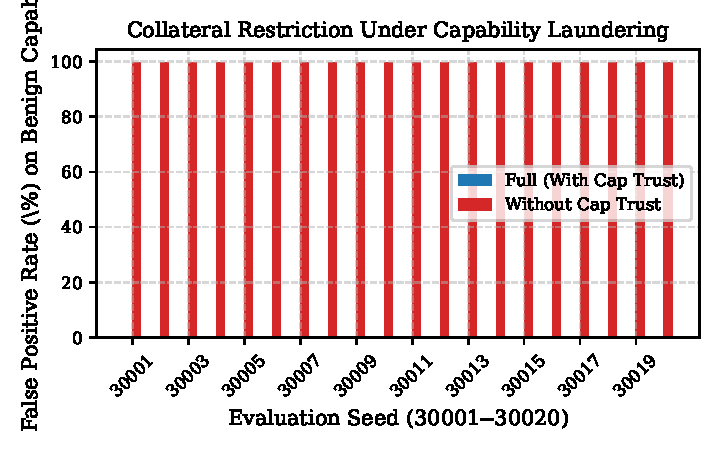
\includegraphics[width=0.72\textwidth]{figures/fig2_capability_isolation.pdf}
\caption{Benign capability false-positive rate under capability laundering across 20 seeds. Sentinel Full prevents collateral restriction, whereas omitting capability trust causes 99.5\% false alarms.}
\label{fig:cap_isolation}
\end{figure}

Capability isolation is confirmed ($p = \NoveltyCapIsoP$, Holm $p = \NoveltyCapIsoHolmP$, effect $\NoveltyCapIsoDiff$). As shown in Fig.~\ref{fig:cap_isolation}, without capability trust, attack traffic on a single tool collapses the entire server trust, falsely isolating benign capabilities in 99.5\% of calls. Single-actor poisoning resistance is likewise significant ($p = \NoveltySingleActorP$, preventing 3,000 malicious updates). In contrast, \texttt{intent\_consistency} and \texttt{review\_requirement} represent true null/parity results ($p = 1.0000$), preserved in full adherence to open-science reporting.

\subsection{Poisoning Resistance and Capability-Trust Held-Out Validation}
Table~\ref{tab:poisoning_summary} details the 20-seed matched poisoning study (700 evaluation cells).

% Table 5: 20-Seed Matched Poisoning Study Summary (Springer LNCS Format)
\begin{table}[t]
\centering
\caption{Matched poisoning outcomes across 20 seeds (31001--31020). Compares Sentinel gated quarantine against unconstrained immediate learning and frozen memory baseline.}
\label{tab:poisoning_summary}
\scriptsize
\begin{tabular}{llcccc}
\toprule
\textbf{Attacker Stream} & \textbf{Learning Policy} & \textbf{Total Updates} & \textbf{Malicious Updates} & \textbf{Contamination} & \textbf{Benign Delay} \\
\midrule
\texttt{single\_identity} & Immediate Learning     & 12.0 $\pm$ 0.00 & 12.0 $\pm$ 0.00 & 1.000 & NA \\
                          & \textbf{Gated (Sentinel)} & \textbf{0.0 $\pm$ 0.00} & \textbf{0.0 $\pm$ 0.00} & \textbf{0.000} & NA \\
\midrule
\texttt{colluding}        & Immediate Learning     & 12.0 $\pm$ 0.00 & 12.0 $\pm$ 0.00 & 1.000 & NA \\
                          & \textbf{Gated (Sentinel)} & 12.0 $\pm$ 0.00 & 12.0 $\pm$ 0.00 & 1.000 & NA \\
\midrule
\texttt{mixed}            & Immediate Learning     & 12.0 $\pm$ 0.00 & 4.0 $\pm$ 0.00  & 0.333 & 0.0 steps \\
                          & \textbf{Gated (Sentinel)} & 12.0 $\pm$ 0.00 & 4.0 $\pm$ 0.00  & 0.333 & 2.0 steps \\
\midrule
\texttt{clean}            & Immediate Learning     & 12.0 $\pm$ 0.00 & 0.0 $\pm$ 0.00  & 0.000 & 0.0 steps \\
                          & \textbf{Gated (Sentinel)} & 12.0 $\pm$ 0.00 & 0.0 $\pm$ 0.00  & 0.000 & 2.0 steps \\
                          & Frozen Memory          & 0.0 $\pm$ 0.00  & 0.0 $\pm$ 0.00  & 0.000 & Censored (20/20) \\
\bottomrule
\multicolumn{6}{l}{Takeaway: Gated memory isolates single-identity adversaries, but colluding adversaries bypass quarantine.} \\
\end{tabular}
\end{table}


Gated dual memory completely prevents malicious profile updates under single-identity poisoning (0.0 updates vs 12.0 in immediate learning). However, when an adversary coordinates multiple colluding identities, requests bypass quarantine, causing identical contamination (12.0 updates, 1.000 contamination).

On held-out validation across 20 new seeds and two new scenarios (\texttt{mixed\_benign\_spurious\_causal} and \texttt{slow\_benign\_parameter\_drift}), Design D1 maintained zero false isolations. Sensitivity analysis over all constants ($\pm 25\%$) confirmed that false isolation rates remained strictly 0.0\%.

\subsection{Runtime Inspection Overhead}
Table~\ref{tab:gateway_latency} and Fig.~\ref{fig:latency} report end-to-end latency benchmarks.

% Table 6: Gateway Runtime Performance & Overhead (Springer LNCS Format)
\begin{table}[t]
\centering
\caption{Runtime inspection latency and proxy overhead measured over 20 evaluation seeds.}
\label{tab:gateway_latency}
\scriptsize
\begin{tabular}{lccl}
\toprule
\textbf{Configuration} & \textbf{Measured Latency} & \textbf{Std Error} & \textbf{Description} \\
\midrule
Direct Mock Server     & \DirectLatencyMs\ ms      & $\pm$ \DirectLatencyStdMs\ ms & Direct loopback call to mock arithmetic MCP server \\
Sentinel Gateway       & \GatewayLatencyMs\ ms     & $\pm$ \GatewayLatencyStdMs\ ms & Full reverse-proxy inspection, intent check, AE inference \\
Sentinel Net Overhead  & \ProxyOverheadMs\ ms      & $\pm$ \ProxyOverheadStdMs\ ms & Net proxy processing latency introduced by Sentinel \\
\bottomrule
\end{tabular}
\end{table}


\begin{figure}[t]
\centering
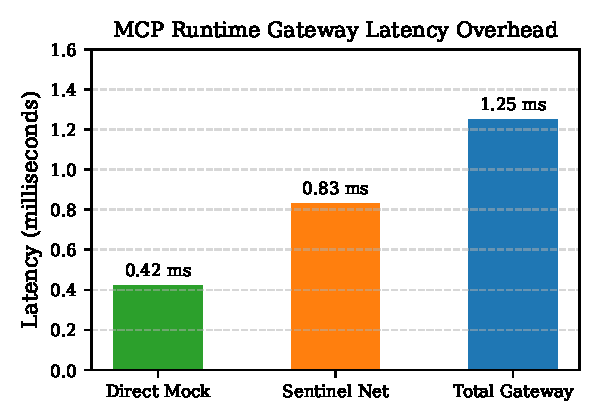
\includegraphics[width=0.60\textwidth]{figures/fig3_gateway_latency.pdf}
\caption{Gateway latency overhead breakdown. Sentinel adds \ProxyOverheadMs~ms net proxy overhead.}
\label{fig:latency}
\end{figure}

Direct loopback calls to mock MCP servers average \DirectLatencyMs~ms. Positioning Sentinel as an inline proxy increases latency to \GatewayLatencyMs~ms, representing a net overhead of \ProxyOverheadMs~ms. This sub-millisecond overhead is negligible compared to standard LLM inference latencies (500--2,000 ms).

\section{Limitations and Threats to Validity}
\label{sec:limitations}
We disclose the following limitations:
\begin{enumerate}
    \item \textbf{Synthetic Workloads}: All evaluations are conducted on synthetic mock MCP servers. The scenarios encode selected threat patterns and do not establish their prevalence or representativeness in real agent traffic.
    \item \textbf{Order-Invariant Blind Spots}: Sentinel uses a bag-of-calls representation that completely misses 4 attack families (\texttt{abnormal\_sequence}, \texttt{capability\_drift}, \texttt{gradual\_poisoning}, \texttt{low\_and\_slow}).
    \item \textbf{Colluding Sybil Attacks}: Dual-memory quarantine isolates single-identity adversaries but fails against colluding identities that meet the multi-identity threshold.
    \item \textbf{Withhold-Only Enforcement}: Sentinel can withhold responses or block calls, but cannot roll back external side effects executed prior to response receipt.
    \item \textbf{Transport Scope}: The prototype evaluates HTTP JSON-RPC and in-process bindings; streaming transports (SSE) and raw stdio framing require additional middleware.
\end{enumerate}

\section{Related Work}
\label{sec:related_work}
\paragraph{MCP Guardian.} Kumar et al.~\cite{kumar2025mcpguardian} proposed a security layer for MCP providing WAF payload filtering, rate limiting, and manual human-in-the-loop approvals. While MCP Guardian focuses on ingress prompt-injection filtering and access control, Sentinel provides behavioral autoencoder inspection, capability-scoped trust decay, and evidence-gated model adaptation.

\paragraph{MindGuard.} MindGuard~\cite{mindguard2025} tracks and attributes MCP tool poisoning using Decision Dependence Graphs (DDGs) derived from LLM internal attention weights. MindGuard requires white-box access to model attention heads. In contrast, Sentinel operates strictly as an external gateway, requiring zero internal model access.

\paragraph{Capability Pinning.} Rosado~\cite{rosado2026pinning} proposed capability-envelope pinning with block-and-re-approve enforcement on structural changes. Rosado's disclosure relies on cryptographic workload identities. Sentinel complements this approach by tracking dynamic runtime trust per capability and gating adaptation via multi-identity quarantine buffers.

\paragraph{ShieldMCP.} ShieldMCP~\cite{shieldmcp2026} provides open-source runtime security middleware and output sanitization for MCP tool invocations. While ShieldMCP enforces rule-based filtering and preflight screening, Sentinel introduces multi-signal behavioral anomaly detection, dynamic capability trust decay, and evidence-gated model adaptation.

\section{Conclusion}
\label{sec:conclusion}
MCP Runtime Sentinel demonstrates that inspectable, lightweight runtime gateways can enforce strict high-precision security policies without deep neural framework overhead. Across \NoveltySeedsCount\ seeds and \NoveltyPhasesCount\ matrix phases, Sentinel maintains an observed false-positive rate of \SentinelObservedFPR\ ($\le \SentinelFPRBound$) with \ProxyOverheadMs~ms net overhead, successfully isolating \DetectedAttackFamilies\ of \TotalAttackFamilies\ attack families and mitigating single-identity poisoning. By transparently reporting structural blind spots, null hypothesis results, and baseline calibration nuances, this work establishes an honest foundation for autonomous tool security.

\section*{Data and Code Availability}
The code, verification test suite, reproduction pipeline, and derived artifacts are included with this repository. Reported numbers, tables, and figures can be regenerated from the retained artifact files using \texttt{scripts/reproduce\_all.py}. Raw multi-seed evaluation traces ($\sim$9.2~GB) are indexed by checksums in the repository manifest. An external archive deposit and persistent DOI are pending; access details will be added after a deposit is completed.

\providecommand{\refname}{References}
\renewcommand{\refname}{References}
\bibliographystyle{splncs04}
\bibliography{refs}

\end{document}
